\documentclass[paper=a4, fontsize=10pt]{scrartcl}

\usepackage{amsmath}
\usepackage[italian]{babel}
\usepackage{tabularx,ragged2e,booktabs,caption} % for table title
\setlength{\parskip}{0.5em} % for paragraph spacing
\DeclareOldFontCommand{\bf}{\normalfont\bfseries}{\mathbf} %declare \bf command in scrartcl

\pagenumbering{gobble} % remove the number of pages

\usepackage{graphicx} % per aggiungere figure/foto

\usepackage{sectsty} % Allows customizing section commands
\allsectionsfont{\normalfont\scshape} % Make all sections, the default font and small caps


%%
\usepackage[utf8]{inputenc}
\newcommand{\approxtext}[1]{\ensuremath{\stackrel{\text{#1}}{\approx}}}
%% now i can add a comment on top of “equal” and “approximate” symbols



\newcommand{\horrule}[1]{\rule{\linewidth}{#1}} % Create horizontal rule command with 1 argument of height

\title{	
\normalfont \normalsize 
\textsc{Universit\`a degli Studi di Trieste - Dipartimento di Ingegneria e Architettura \\ Ingegneria elettronica e informatica - Applicazioni informatiche} \\ [25pt] % Your university, school and/or department name(s)
\horrule{0.5pt} \\[0.4cm] % Thin top horizontal rule
\huge \textbf{Relazione progetto Reti Logiche\\ Weather Station}  \\ % The assignment title
\horrule{2pt} \\[0.5cm] % Thick bottom horizontal rule
}

\author{Andrea Gonzato} % Your name

\date{\normalsize 30 Maggio 2019} % Today's date or a custom date

\setlength{\parindent}{0cm}

\begin{document}
\maketitle % Print the title

\pagebreak

\tableofcontents

\pagebreak

\section{Introduzione}
La relazione riguarda il progetto di Arduino svolto per il corso di reti logiche, tenuto dal professor Marsi dell'Università di Trieste.

\section{Scopo del progetto}
Lo scopo del progetto "Weather Station", come suggerisce il nome, è quello di realizzare una stazione meteorologica amatoriale. L'obiettivo principale è di poter visualizzare la temperatura e l'umidità attuale. Funzionalità secondarie richieste sono: la possibilità di poter leggere l'ora, la data e di poter utilizzare la stazione anche come sveglia. Inoltre è previsto che data, ora e sveglia siano regolabili e che questa sia disattivabile.

\subsection{Descrizione per l'utilizzo}
Per controllare la stazione meteorologica ci sono tre pulsanti: \textit{SET}, \textbf{+}, \textbf{-}.
Il funzionamento ricorda molto l'utilizzo dei classici orologi da polso digitali. Dunque per poter scorrere tutte le funzionalità si utilizzano i pulsanti \textbf{+} e \textbf{-}, mentre per impostare la data, l'ora e la sveglia bisogna tenere premuto, per un secondo, il pulsante \textit{SET}; dopodiché per la regolazione si usano gli analoghi pulsanti,  \textbf{+} e \textbf{-}; invece per passare ad impostare il campo successivo o per attivare/disattivare la sveglia bisogna premere il pulsante \textit{SET} una singola volta.


\subsection{Specifiche}
Il progetto esige come prima specifica che l'orologio non necessiti di una regolazione più di una volta al mese. 
Si richiede quindi la sincronizzazione con un orologio affidabile e dopo 24 ore ci dev'essere una differenza non superiore a un secondo.

La seconda specifica, sui dati meteo, chiede un errore inferiore ad 1 grado Celsius per la temperatura e 2 punti percentuali per l'umidità.

\subsection{Risultato ottenuto}
Nella figura \ref{fig:progettoFoto} si può vedere la realizzazione del progetto completo.

Tutte le specifiche per la realizzazione finale del progetto sono state rispettate.

Nel complesso il sistema si può ritenere funzionante, stabile e facile all'uso.

\begin{figure}
  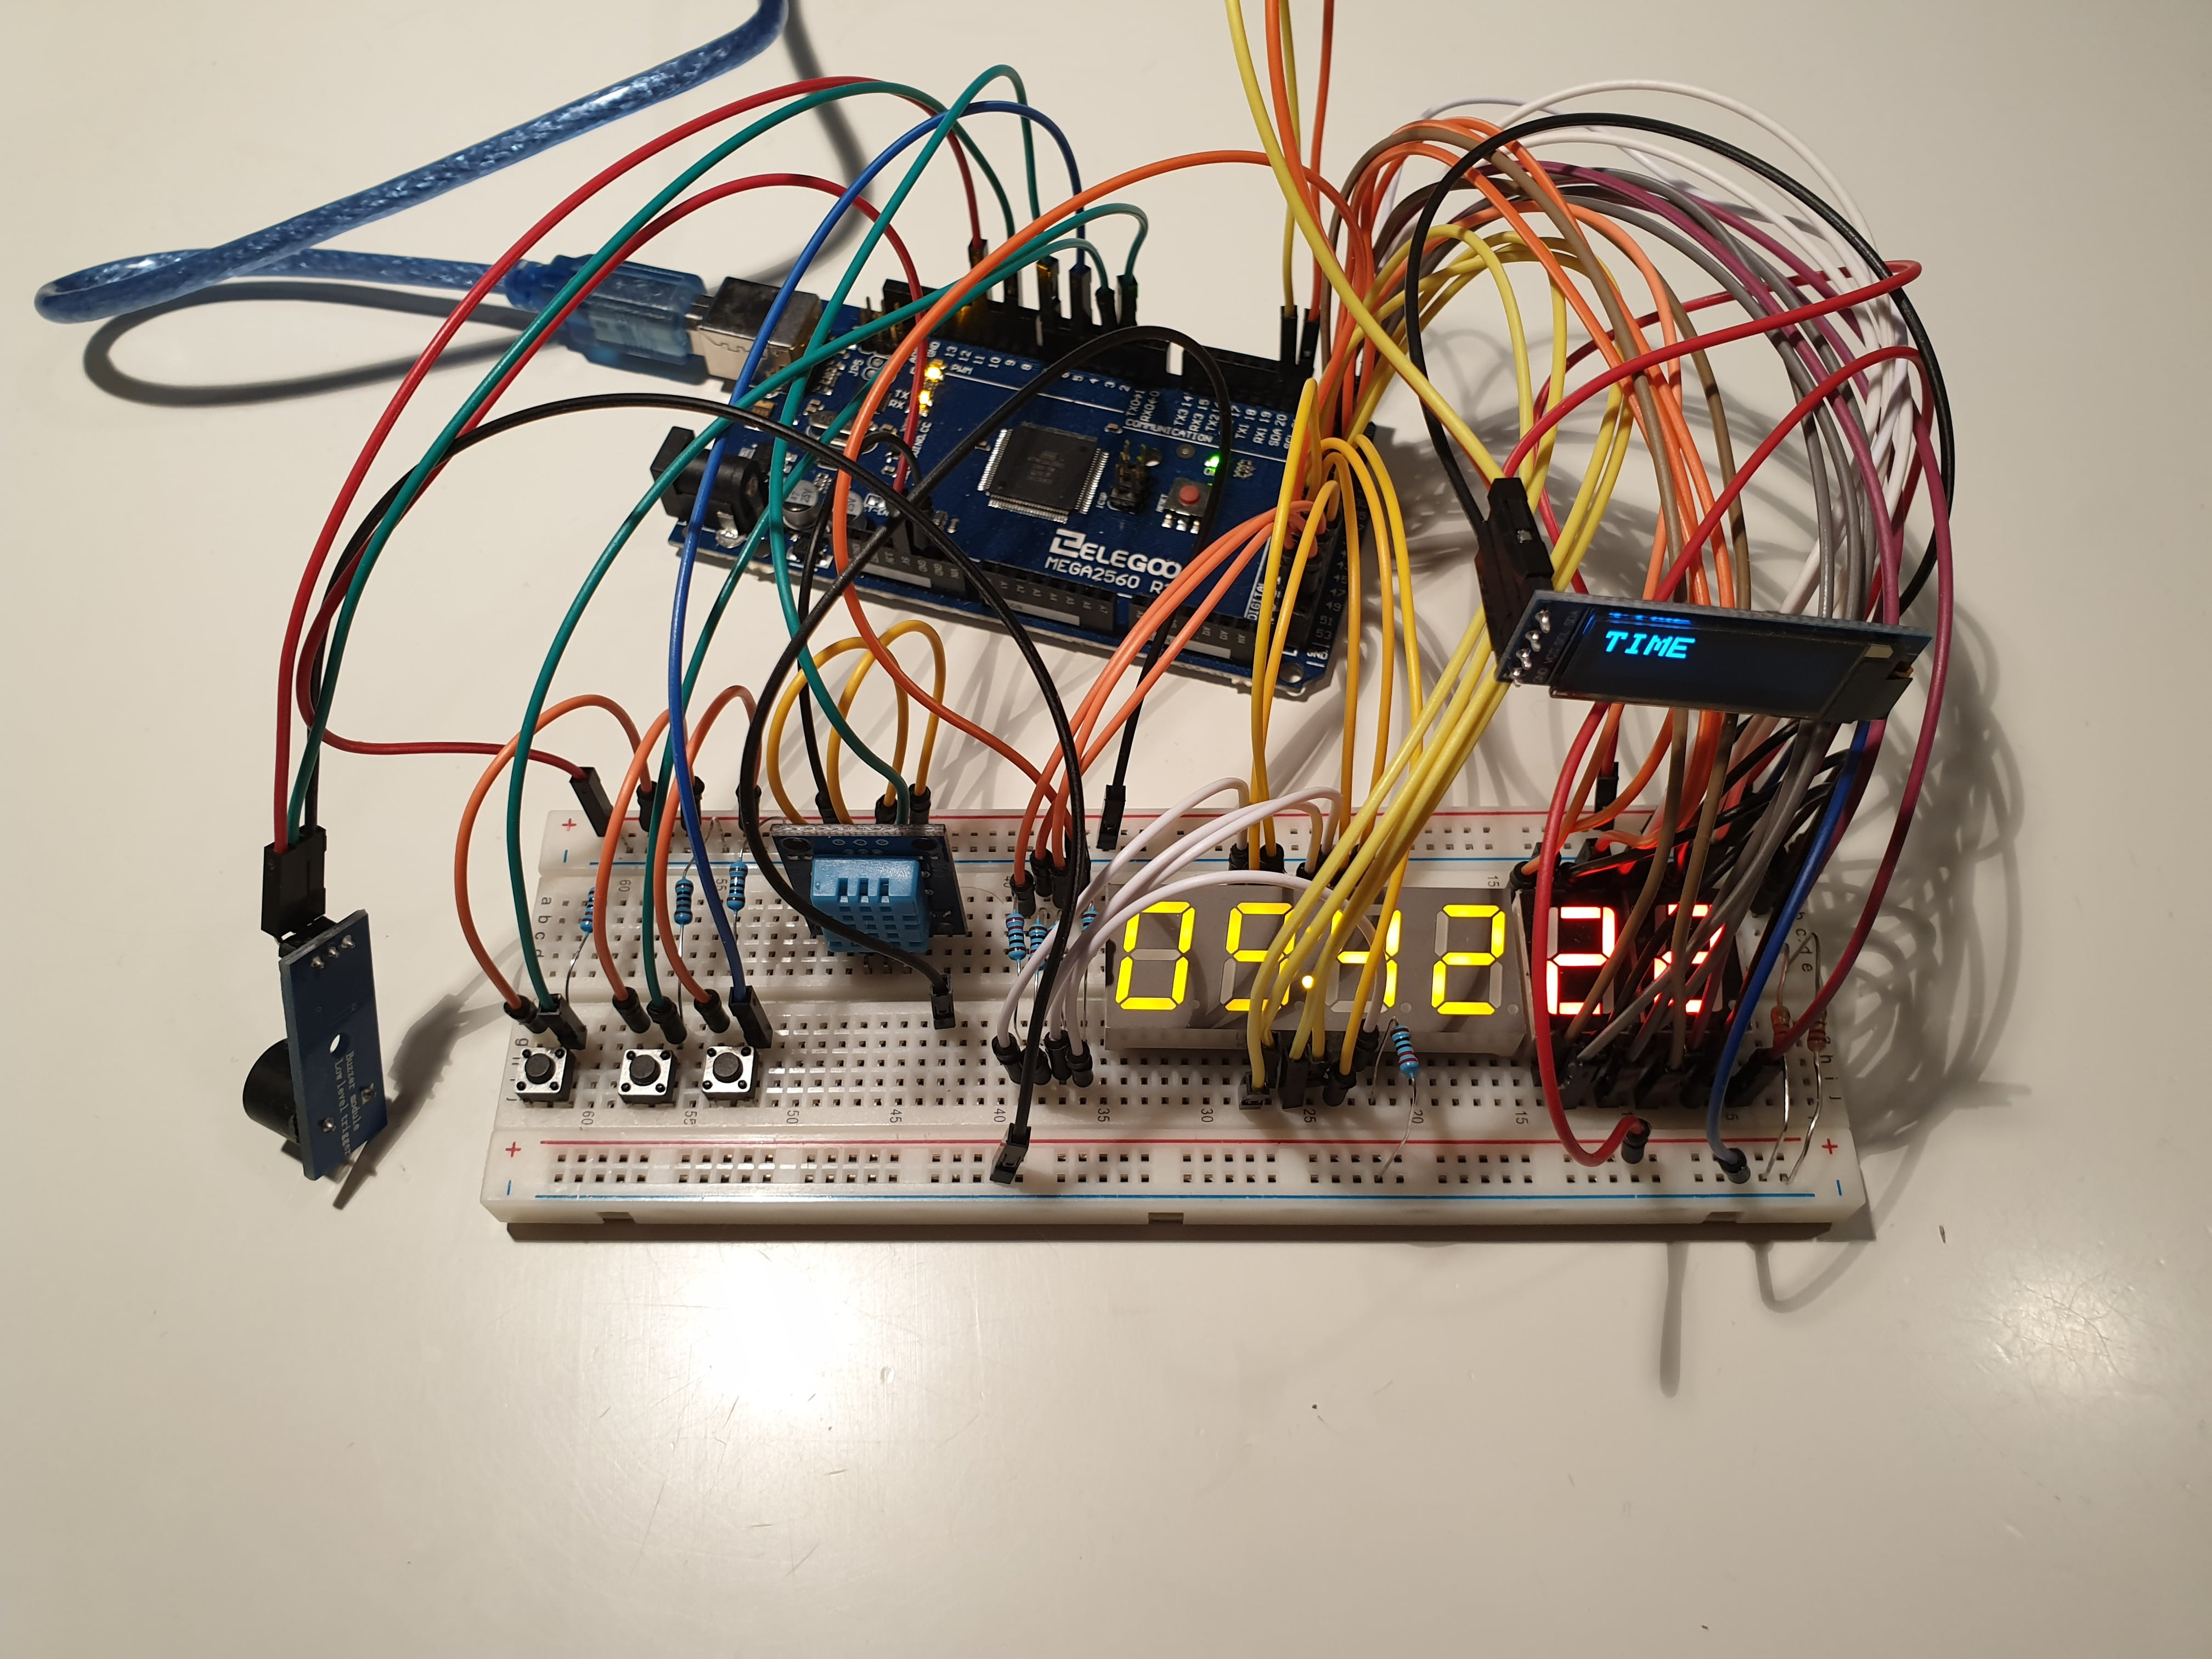
\includegraphics[scale=0.05]{projectPhoto.jpg}
  \caption{una immagine del progetto}
  \label{fig:progettoFoto}
\end{figure}
    

\section{Realizzazione}
Il progetto è stato realizzato tra Marzo 2019 e Maggio 2019.\\

\subsection{Metodo usato}
In una prima fase, reperiti i componenti si sono eseguiti una serie di test per comprendere l'utilizzo e le capacità dei singoli.

Nella seconda fase, momento in cui è iniziata la vera realizzazione del progetto, la metodologia adottata si è ispirata al paradigma AGILE. Seguendo questa metodologia si aggiungono funzionalità, una alla volta, passando ciclicamente da una fase di progettazione a una di sviluppo per poi passare ai test e verificare la correttezza delle implementazioni eseguite.

\begin{figure}
  
\includegraphics[scale=0.2]{AGILE.jpeg}
  \caption{paradigma AGILE}
  \label{fig:agile1}
\end{figure}
    
La figura \ref{fig:agile1}
illustra bene il paradigma adottato.


Nell'ultima fase del progetto, una volta implementate gran parte delle funzionalità, bisogna ristrutture il codice, creando una nuova versione strutturata ad oggetti, per poter avere un codice più leggibile ed uniforme.

\pagebreak

\subsection{Struttura della programmazione ad oggetti implementata}
Di seguito viene fornita una breve descrizione di come è stato strutturato ad oggetti il progetto.

Tutti gli oggetti vengono creati nel file \textit{Code/code.ino} e per ogni classe viene implementato un solo oggetto, a parte per la classe \textit{Button} dove ne vengono creati tre. I metodi "principali" di ogni classe si chiamano \textit{update()} e in tali metodi i vari oggetti comunicano tra di loro, i cambiamenti registrati durante il ciclo di esecuzione della funzione \textit{loop()}.

Le classi implementate sono:

\begin{itemize}
\item MyTime: una classe che contiene tutte le variabili temporali e scandisce nel tempo l'evoluzione del sistema. Questa classe serve, per esempio, per l'attivazione dell'allarme della sveglia.

\item Mode: una classe che gestisce e aggiorna il sistema informandolo su cosa bisogna visualizzare sui display a 7 segmenti. Nella stazione meteo ci sono 5 dati fondamentali da far vedere all'utente che sono: il tempo, la data, la temperatura, l'umidità e l'orario al quale è impostata la sveglia. Ma si noti che per questioni progettuali solo uno alla volta di questi dati può essere visualizzato sui display.

\item Button: una classe che gestisce tutte le attività che iniziano alla pressione di un pulsante, per esempio, aggiorna il sistema comunicando che durante un settaggio si è premuto un pulsante per far aumentare le ore dell'orologio. Questa classe è in continua comunicazione con MyTime e Mode.

\item ControllSingleDigitDisplay: una classe che si occupa di visualizzare i dati richiesti sui 2 display a 7 segmenti 1 digit.
\end{itemize}


\subsection{Componenti utilizzati}
Questa è una lista completa del materiale utilizzato
\begin{itemize}
\item Arduino Mega 2560
\item breadboard (63x10)
\item sensore digitale DHT11 per rilevare temperatura e umidità
\item schermo OLED (risoluzione: 128*32)
\item display 7 segmenti (4 digits, catodo comune)
\item 2 display 7 segmenti (1 digit, catodo comune)
\item cicalino (buzzer passivo)
\item 3 bottoni
\item 7 resistenze da 220 Ohm
\item 3 resistenze da 1k Ohm
\item 50/55 cavi elettrici M/M
\item 8 cavi elettrici M/F
\end{itemize}

Si osservi che per la realizzazione di questo progetto non è sufficiente un Arduino Uno, perché da come si vede in Figura \ref{fig:schema1}, sono necessarie 34 connessioni digitali.
\subsection{Schema}
In fondo alla relazione si può osservare la figura \ref{fig:schema1} che indica lo schema utilizzato per il progetto.

Si nota che nello schema non sono presenti le connessioni del cicalino e dello schermo OLED. Queste sono particolarmente semplici e intuitive. Se si vuole usare il codice del progetto, i pin del cicalino I/O e VCC vanno connessi rispettivamente a i pin Arduino 9 e 11.

\pagebreak

\subsection{Strumenti usati}
I principali strumenti utilizzati sono: l'ambiente Arduino e Fritzing come software per disegnare gli schemi elettronici.\\
Nel codice del progetto sono presenti come librerie esterne:
\begin{itemize}
\item \textit{SevSeg}
\item \textit{DHT}
\item \textit{Adafruit Sensor}
\item \textit{Adafruit GFX}
\item \textit{Adafruit SSD1306}
\end{itemize}

\textit{SevSeg} è utile per "scrivere" sul display a 7 segmenti 4 digits; mentre \textit{DHT} e \textit{Adafruit Sensor} servono per leggere i dati dal sensore che rilevava la temperatura e l'umidità; infine  le ultime due librerie permettono di utilizzare lo schermo OLED. 


\subsection{Scelte progettuali e difficoltà}
Una delle scelte progettuali fondamentali è quella di decidere come far scandire il tempo al sistema:
Una possibilità consiste nell'acquistare un modulo RTC appositamente designato per queste attività. In alternativa si può far scandire il tempo direttamente ad Arduino. Infatti si può creare una variabile \textit{long unsigned} che si incrementa al passare di ogni millisecondo. Se si sceglie quest'ultima realizzazione, che è quella attuata nel progetto, si evita l'acquisto di un modulo, ma il prezzo da pagare è un potenziale crash di sistema. Infatti, teoricamente, dopo 4,294,967,295 millisecondi, cioè circa 49 giorni, la variabile arriva in \textit{overflow}. Questo avvenimento non è ancora stato testato, ma si raccomanda di resettare la stazione prima dello scadere del quarantottesimo giorno dall'avvio.

La difficoltà più grande, che si incontra durante il progetto, è sicuramente la gestione e la sincronizzazione dei display a 7 segmenti. Nel progetto di partenza, l'idea era quella di realizzare un sistema di visualizzazione dati, utilizzando due display a 7 segmenti con 4 digits, quindi poter disporre di un totale di 8 digits. Il problema di questa realizzazione è che la libreria \textit{SevSeg} utilizzata non supporta l'opportunità di comandare più display contemporaneamente. Il progetto finale si realizza con l'implementazione di un display 4 digits, controllato dalla libreria, affiancato da due display sigle digit, controllati senza libreria, ma con comandi standard \textit{digitalWrite()} di Arduino. Questa realizzazione rende l'aggiornamento dei display non uniforme e non ottimizzata, infatti ad ogni esecuzione dell'\textit{loop()}, ciclicamente un solo digit del display, composto da quattro digit, si aggiorna mentre entrambi i display single digit si aggiornano contemporaneamente. In futuro, si potrebbe migliorare questa non uniformità nell'illuminazione dei display, ma attualmente non si ritiene fondamentale.

Come protocollo di comunicazione tra il display OLED e Arduino viene usato il protocollo $I^{2}C$. La motivazione di questa scelta risiede dal fatto, che l'Arduino Mega 2560 possiede due pin, addetti a tale scopo.

L'utilizzo della libreria \textit{SevSeg} porta che all'interno del \textit{loop()} non può essere inserito alcun ritardo di qualunque tipo. Se si verificassero questi ritardi, il display a 7 segmenti 4 digits inizierebbe a sfarfallare. A causa di questa problematica il sensore di umidità e temperatura rileva i dati non in maniera continuata, ma esclusivamente ogni 20 secondi. Questo avviene perché se no si verificherebbero dei ritardi nell'\textit{loop()}. Infatti, se si osserva bene il display, ogni 20 secondi, c'è un piccolo sfarfallamento, ma non è particolarmente fastidioso.



\section{Sviluppi futuri}
I prossimi sviluppi per questo progetto riguardano aspetti secondari.
Di seguito vengono elencate alcuni possibili sviluppi futuri per il progetto:
\begin{itemize}
\item introduzione di nuove melodie più piacevoli per la sveglia.

\item introduzione di una nuova funzionalità che permetta l'uso della stazione anche come cronometro.

\item introduzione di una nuova funzionalità che permetta l'uso della stazione anche come timer.

\item implementazione di un sensore che rilevi la pressione (barometro) e di una funzionalità che permetta di vedere il suo stato attuale.

\item introduzione di effetti sonori, durante le attività di settaggio degli strumenti.

\item implementazione di un sistema di memorizzazione che scriva i dati meteorologici (temperatura, umidità e pressione) in una scheda sd, permettendo di creare degli storici sui dati rilevati.

\end{itemize}


\section{Rilascio materiale}
Tutto il materiale di questo progetto è rilasciato con licenza open source ed è reperibile al seguente sito:
\textit{https://github.com/AndreaGonzato/WeatherStation}

In questa pagina è possibile trovare anche la vecchia versione del codice non strutturato ad oggetti. Tale versione, chiamata \textit{"Code No OOP"}, non supporta le ultime funzionalità come ad esempio la sveglia. Questa versione può rilevarsi utile per chi intende contribuire a questo progetto, ma non ha molta famigliarità con la programmazione ad oggetti.


\section{Conclusioni}
Sicuramente il progetto non è ne perfetto ne completo, ma nel complesso si può definire un prototipo funzionante.

\section{Sitografia}

Le librerie utilizzate sono reperibili ai seguenti siti:
\begin{itemize}
\item https://github.com/DeanIsMe/SevSeg
\item https://github.com/adafruit/Adafruit-GFX-Library
\item https://github.com/adafruit/Adafruit\_SSD1306
\item https://github.com/adafruit/DHT-sensor-library
\item https://github.com/adafruit/Adafruit\_Sensor
\end{itemize}

Altri siti dove sono state lette guide e tutorial sono:
\begin{itemize}
\item https://www.arduino.cc/en/Tutorial/BuiltInExamples
\item https://create.arduino.cc/projecthub
\item http://www.circuitbasics.com/arduino-7-segment-display-tutorial/
\item https://overvolt.tech/sensori/3
\item http://www.associazionemarconi.com/calcolo/codice\_resistenze\_elettriche\_5.html
\end{itemize}


\section{Dichiarazione finale}
Tutto il lavoro è stato svolto da me in completa autonomia.

\begin{figure}
  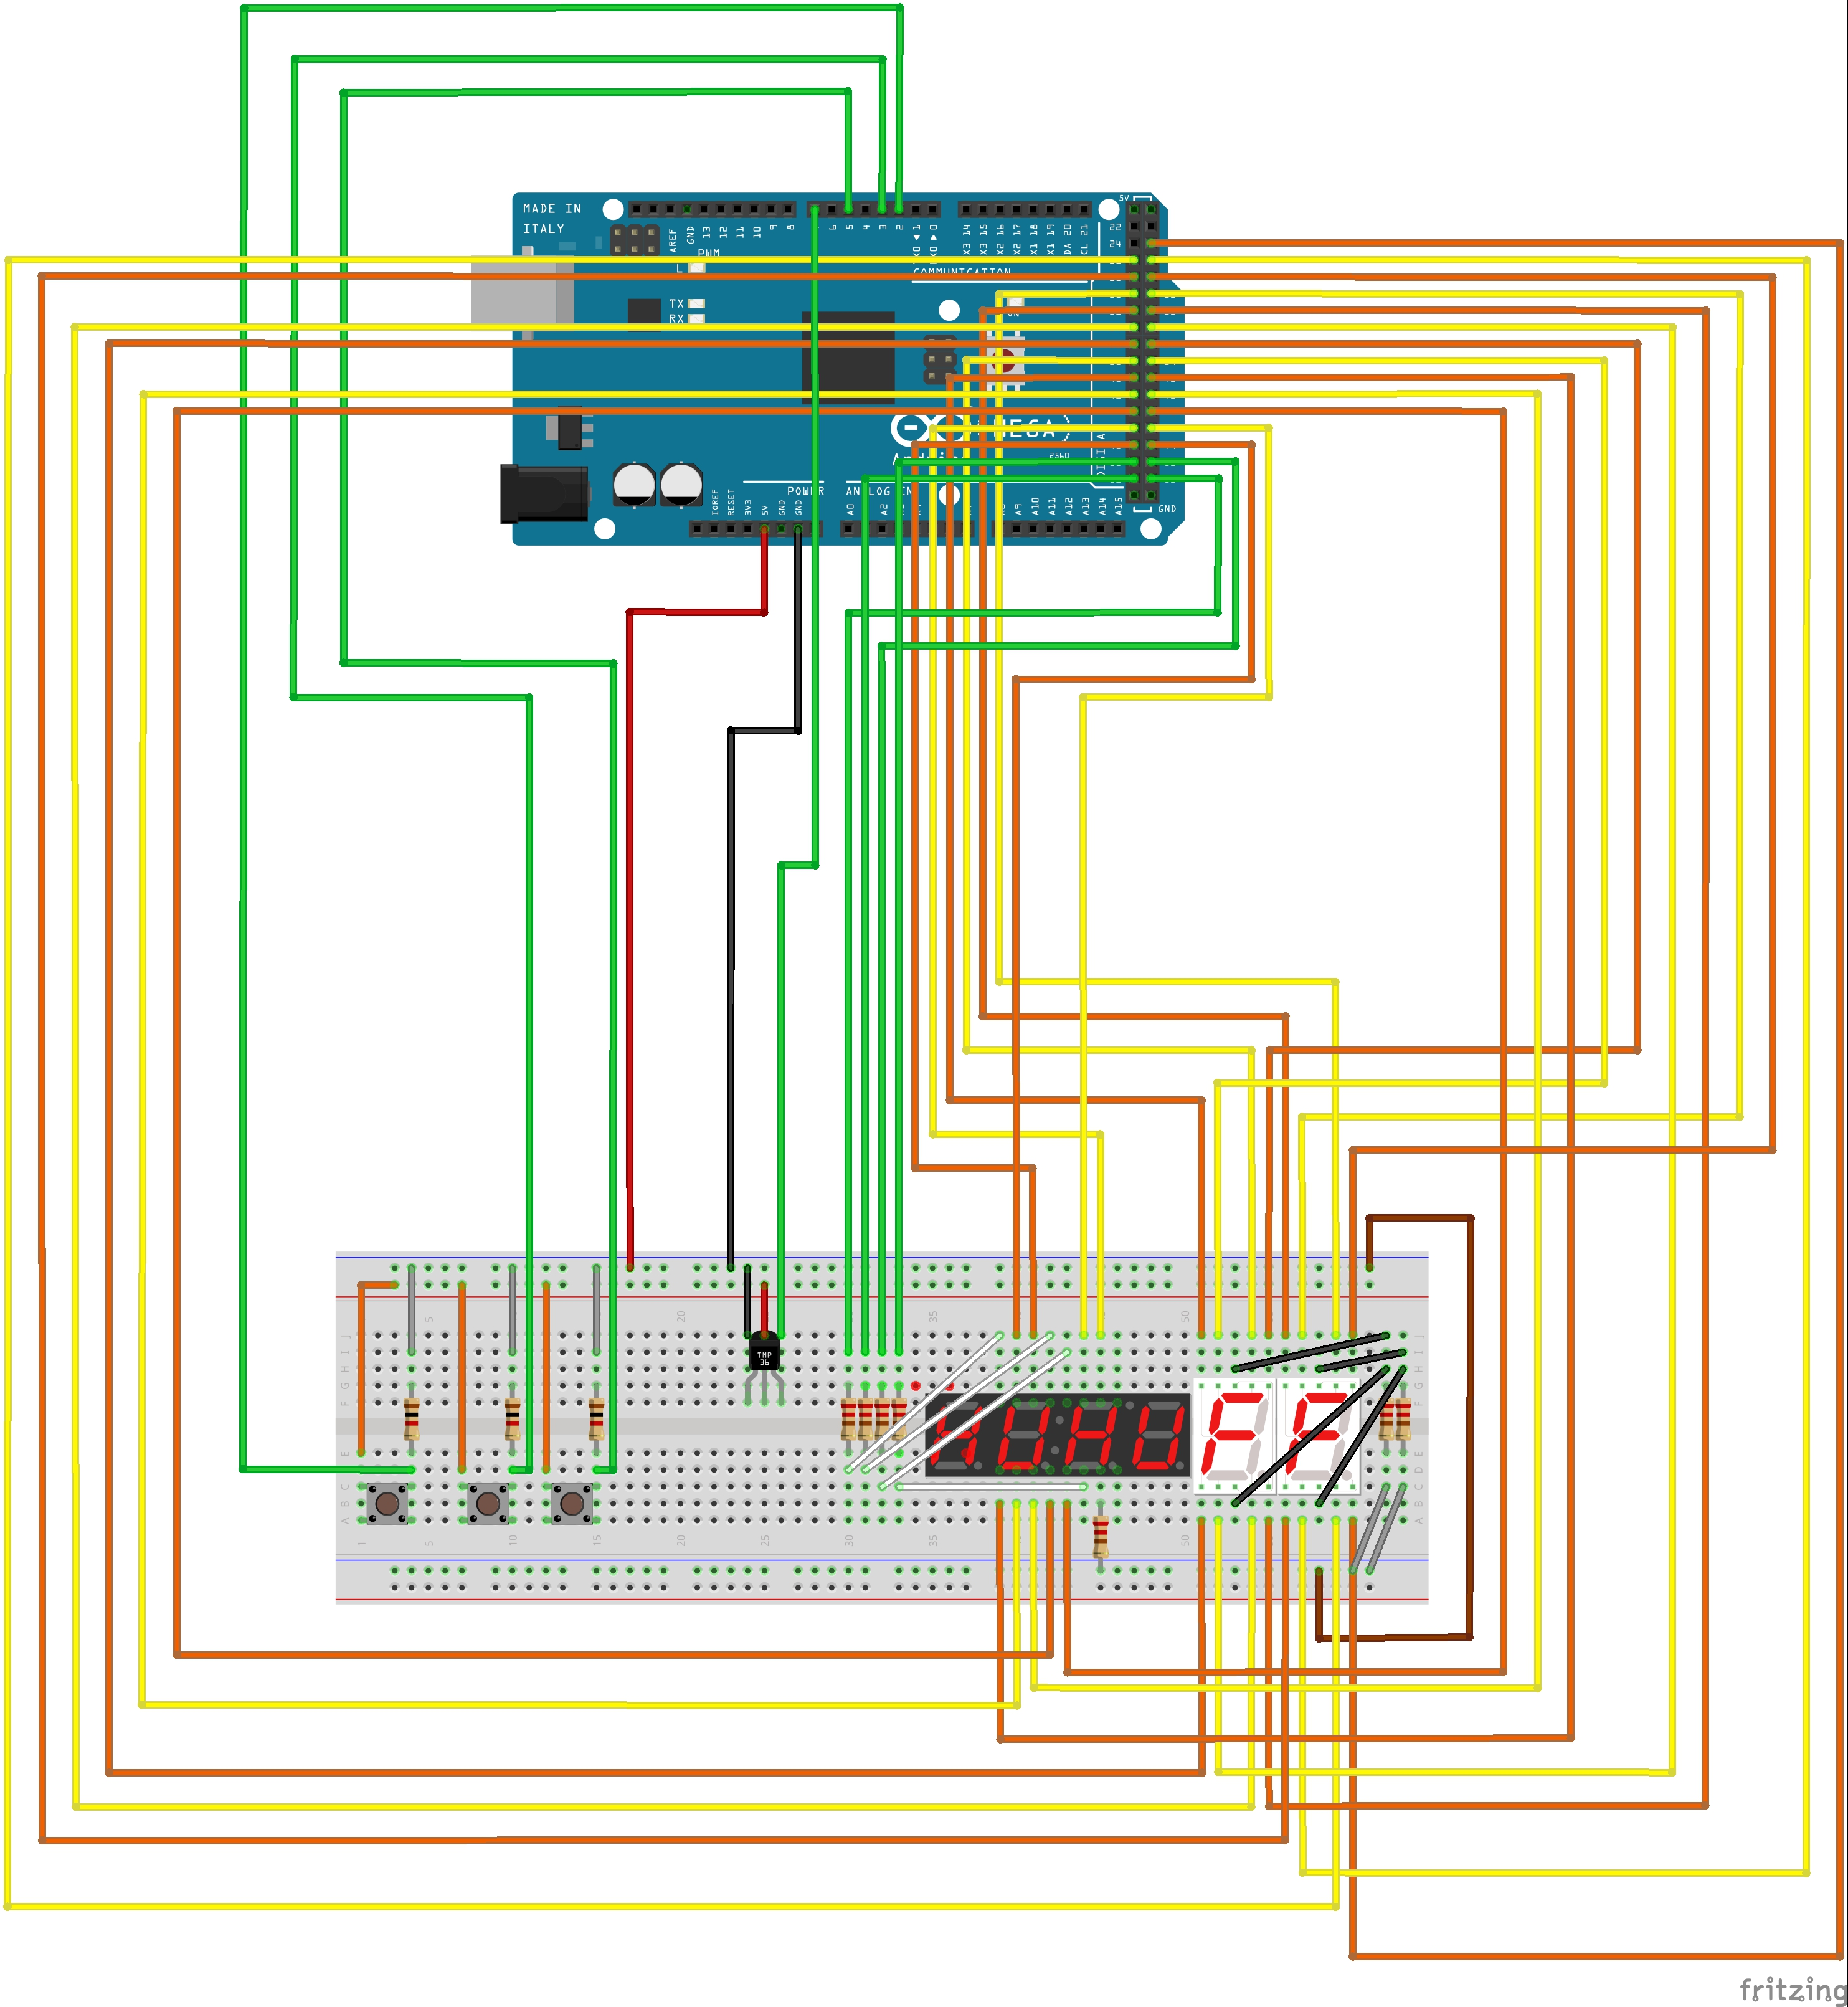
\includegraphics[width=\linewidth]{MySchema.jpg}
  \caption{Schema del circuito}
  \label{fig:schema1}
\end{figure}

\end{document}